%% fig_cmsource.tex   (generated by make_round19.py; do not edit by hand)
%% The 132 Hodge classes of degree four on the square at a CM point: 100 products of divisor classes, 32 tetrahedron monomials, the ten symmetric sums, and the coefficients of s_{+,2} and of pi_12 - pi_13 on the six mixed monomials of T_+ (prop:cmsource).
\documentclass[tikz,border=8pt]{standalone}
\usepackage{amsmath,amssymb}
\usetikzlibrary{arrows.meta,calc,decorations.pathreplacing}
%% palette.tex -- shared colour definitions for the figures
\definecolor{PInk}{RGB}{26,32,44}
\definecolor{PBlue}{RGB}{37,82,139}
\definecolor{PTeal}{RGB}{23,127,125}
\definecolor{POchre}{RGB}{193,138,44}
\definecolor{PClay}{RGB}{178,74,58}
\definecolor{PSlate}{RGB}{108,122,137}
\definecolor{PViolet}{RGB}{110,86,150}
\definecolor{WBlue}{RGB}{223,234,246}
\definecolor{WTeal}{RGB}{220,238,236}
\definecolor{WOchre}{RGB}{250,240,218}
\definecolor{WClay}{RGB}{247,229,224}
\definecolor{WSlate}{RGB}{238,241,244}
\definecolor{PMag}{RGB}{158,58,110}
\definecolor{PGrass}{RGB}{62,124,66}
\definecolor{PAmber}{RGB}{214,112,38}
\definecolor{PIndigo}{RGB}{58,64,140}
\definecolor{PRule}{RGB}{176,186,197}

%% shared macros so the standalone figures match the paper
\providecommand{\QQ}{\mathbb{Q}}
\providecommand{\ZZ}{\mathbb{Z}}
\providecommand{\RR}{\mathbb{R}}
\providecommand{\CC}{\mathbb{C}}
\providecommand{\PP}{\mathbb{P}}
\providecommand{\Kx}{K^{\times}}
\providecommand{\HW}{W}
\providecommand{\Nm}{\mathrm{N}}
\providecommand{\Hdg}{\mathrm{Hdg}}
\providecommand{\NS}{\mathrm{NS}}
\providecommand{\cA}{\mathcal{A}}
\providecommand{\cD}{\mathcal{D}}
\providecommand{\cF}{\mathcal{F}}
\providecommand{\cP}{\mathcal{P}}
\providecommand{\cO}{\mathcal{O}}
\providecommand{\cQ}{\mathcal{Q}}
\providecommand{\bbar}[1]{\overline{#1}}
\providecommand{\ch}{\operatorname{ch}}
\providecommand{\End}{\mathrm{End}}
\providecommand{\Ext}{\operatorname{Ext}}
\providecommand{\Supp}{\operatorname{Supp}}

\begin{document}
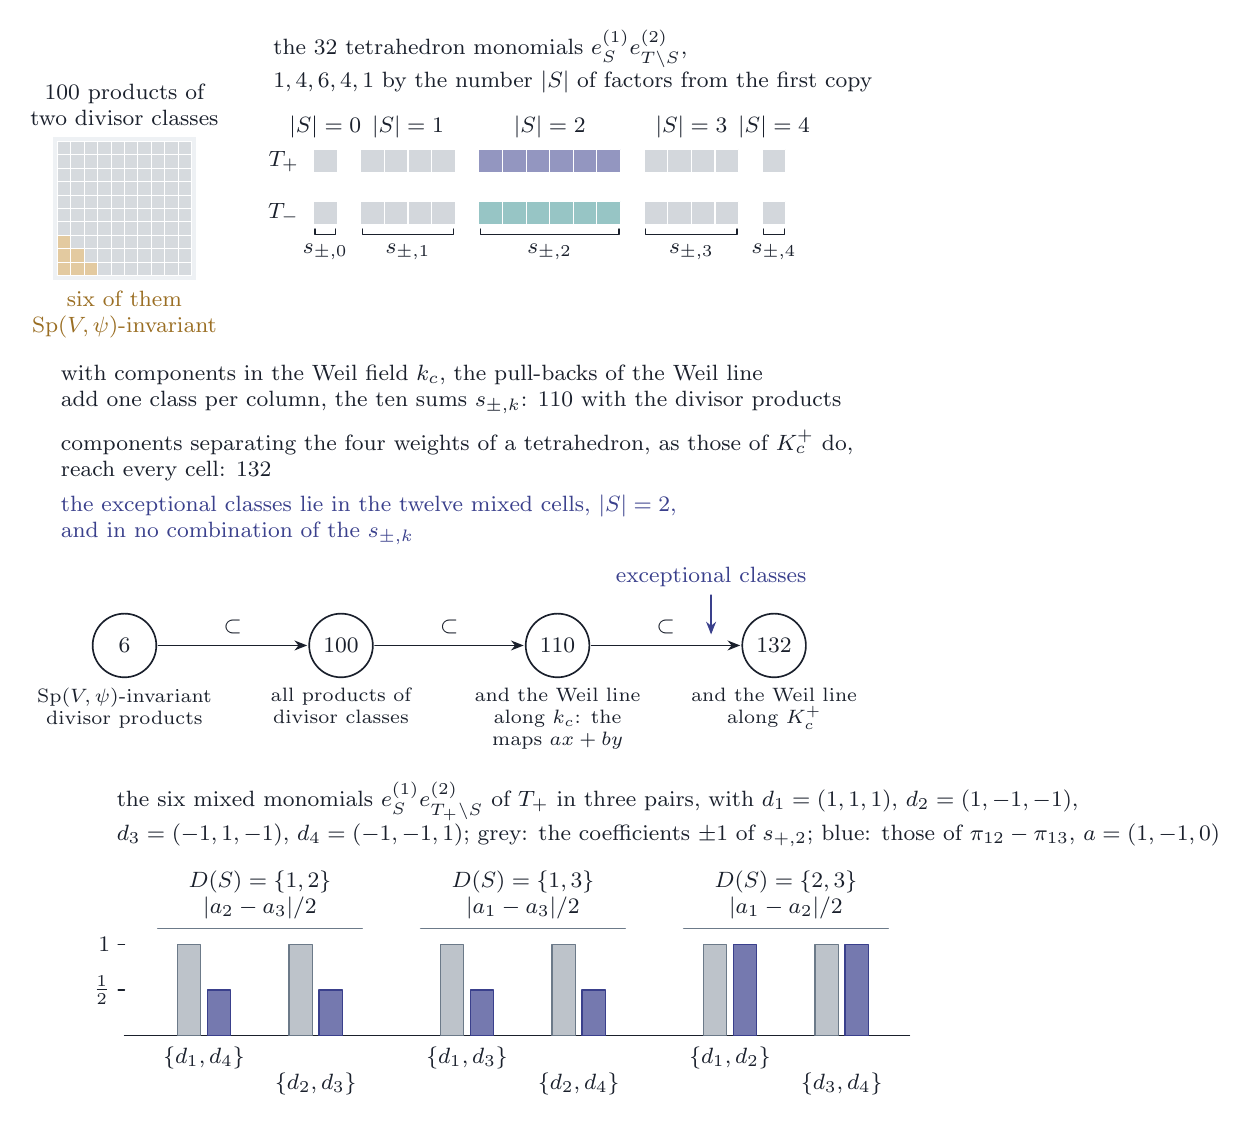
\begin{tikzpicture}[x=1cm,y=1cm,line join=round,line cap=round,
  font=\small,text=PInk,lbl/.style={inner sep=1pt}]
  \path[fill=WSlate,draw=none] (-0.0600,-0.0600) rectangle (1.7600,1.7600);
  \path[fill=POchre!45!white,draw=white,line width=0.35pt] (0.0000,0.0000) rectangle (0.1700,0.1700);
  \path[fill=POchre!45!white,draw=white,line width=0.35pt] (0.1700,0.0000) rectangle (0.3400,0.1700);
  \path[fill=POchre!45!white,draw=white,line width=0.35pt] (0.3400,0.0000) rectangle (0.5100,0.1700);
  \path[fill=PSlate!28!white,draw=white,line width=0.35pt] (0.5100,0.0000) rectangle (0.6800,0.1700);
  \path[fill=PSlate!28!white,draw=white,line width=0.35pt] (0.6800,0.0000) rectangle (0.8500,0.1700);
  \path[fill=PSlate!28!white,draw=white,line width=0.35pt] (0.8500,0.0000) rectangle (1.0200,0.1700);
  \path[fill=PSlate!28!white,draw=white,line width=0.35pt] (1.0200,0.0000) rectangle (1.1900,0.1700);
  \path[fill=PSlate!28!white,draw=white,line width=0.35pt] (1.1900,0.0000) rectangle (1.3600,0.1700);
  \path[fill=PSlate!28!white,draw=white,line width=0.35pt] (1.3600,0.0000) rectangle (1.5300,0.1700);
  \path[fill=PSlate!28!white,draw=white,line width=0.35pt] (1.5300,0.0000) rectangle (1.7000,0.1700);
  \path[fill=POchre!45!white,draw=white,line width=0.35pt] (0.0000,0.1700) rectangle (0.1700,0.3400);
  \path[fill=POchre!45!white,draw=white,line width=0.35pt] (0.1700,0.1700) rectangle (0.3400,0.3400);
  \path[fill=PSlate!28!white,draw=white,line width=0.35pt] (0.3400,0.1700) rectangle (0.5100,0.3400);
  \path[fill=PSlate!28!white,draw=white,line width=0.35pt] (0.5100,0.1700) rectangle (0.6800,0.3400);
  \path[fill=PSlate!28!white,draw=white,line width=0.35pt] (0.6800,0.1700) rectangle (0.8500,0.3400);
  \path[fill=PSlate!28!white,draw=white,line width=0.35pt] (0.8500,0.1700) rectangle (1.0200,0.3400);
  \path[fill=PSlate!28!white,draw=white,line width=0.35pt] (1.0200,0.1700) rectangle (1.1900,0.3400);
  \path[fill=PSlate!28!white,draw=white,line width=0.35pt] (1.1900,0.1700) rectangle (1.3600,0.3400);
  \path[fill=PSlate!28!white,draw=white,line width=0.35pt] (1.3600,0.1700) rectangle (1.5300,0.3400);
  \path[fill=PSlate!28!white,draw=white,line width=0.35pt] (1.5300,0.1700) rectangle (1.7000,0.3400);
  \path[fill=POchre!45!white,draw=white,line width=0.35pt] (0.0000,0.3400) rectangle (0.1700,0.5100);
  \path[fill=PSlate!28!white,draw=white,line width=0.35pt] (0.1700,0.3400) rectangle (0.3400,0.5100);
  \path[fill=PSlate!28!white,draw=white,line width=0.35pt] (0.3400,0.3400) rectangle (0.5100,0.5100);
  \path[fill=PSlate!28!white,draw=white,line width=0.35pt] (0.5100,0.3400) rectangle (0.6800,0.5100);
  \path[fill=PSlate!28!white,draw=white,line width=0.35pt] (0.6800,0.3400) rectangle (0.8500,0.5100);
  \path[fill=PSlate!28!white,draw=white,line width=0.35pt] (0.8500,0.3400) rectangle (1.0200,0.5100);
  \path[fill=PSlate!28!white,draw=white,line width=0.35pt] (1.0200,0.3400) rectangle (1.1900,0.5100);
  \path[fill=PSlate!28!white,draw=white,line width=0.35pt] (1.1900,0.3400) rectangle (1.3600,0.5100);
  \path[fill=PSlate!28!white,draw=white,line width=0.35pt] (1.3600,0.3400) rectangle (1.5300,0.5100);
  \path[fill=PSlate!28!white,draw=white,line width=0.35pt] (1.5300,0.3400) rectangle (1.7000,0.5100);
  \path[fill=PSlate!28!white,draw=white,line width=0.35pt] (0.0000,0.5100) rectangle (0.1700,0.6800);
  \path[fill=PSlate!28!white,draw=white,line width=0.35pt] (0.1700,0.5100) rectangle (0.3400,0.6800);
  \path[fill=PSlate!28!white,draw=white,line width=0.35pt] (0.3400,0.5100) rectangle (0.5100,0.6800);
  \path[fill=PSlate!28!white,draw=white,line width=0.35pt] (0.5100,0.5100) rectangle (0.6800,0.6800);
  \path[fill=PSlate!28!white,draw=white,line width=0.35pt] (0.6800,0.5100) rectangle (0.8500,0.6800);
  \path[fill=PSlate!28!white,draw=white,line width=0.35pt] (0.8500,0.5100) rectangle (1.0200,0.6800);
  \path[fill=PSlate!28!white,draw=white,line width=0.35pt] (1.0200,0.5100) rectangle (1.1900,0.6800);
  \path[fill=PSlate!28!white,draw=white,line width=0.35pt] (1.1900,0.5100) rectangle (1.3600,0.6800);
  \path[fill=PSlate!28!white,draw=white,line width=0.35pt] (1.3600,0.5100) rectangle (1.5300,0.6800);
  \path[fill=PSlate!28!white,draw=white,line width=0.35pt] (1.5300,0.5100) rectangle (1.7000,0.6800);
  \path[fill=PSlate!28!white,draw=white,line width=0.35pt] (0.0000,0.6800) rectangle (0.1700,0.8500);
  \path[fill=PSlate!28!white,draw=white,line width=0.35pt] (0.1700,0.6800) rectangle (0.3400,0.8500);
  \path[fill=PSlate!28!white,draw=white,line width=0.35pt] (0.3400,0.6800) rectangle (0.5100,0.8500);
  \path[fill=PSlate!28!white,draw=white,line width=0.35pt] (0.5100,0.6800) rectangle (0.6800,0.8500);
  \path[fill=PSlate!28!white,draw=white,line width=0.35pt] (0.6800,0.6800) rectangle (0.8500,0.8500);
  \path[fill=PSlate!28!white,draw=white,line width=0.35pt] (0.8500,0.6800) rectangle (1.0200,0.8500);
  \path[fill=PSlate!28!white,draw=white,line width=0.35pt] (1.0200,0.6800) rectangle (1.1900,0.8500);
  \path[fill=PSlate!28!white,draw=white,line width=0.35pt] (1.1900,0.6800) rectangle (1.3600,0.8500);
  \path[fill=PSlate!28!white,draw=white,line width=0.35pt] (1.3600,0.6800) rectangle (1.5300,0.8500);
  \path[fill=PSlate!28!white,draw=white,line width=0.35pt] (1.5300,0.6800) rectangle (1.7000,0.8500);
  \path[fill=PSlate!28!white,draw=white,line width=0.35pt] (0.0000,0.8500) rectangle (0.1700,1.0200);
  \path[fill=PSlate!28!white,draw=white,line width=0.35pt] (0.1700,0.8500) rectangle (0.3400,1.0200);
  \path[fill=PSlate!28!white,draw=white,line width=0.35pt] (0.3400,0.8500) rectangle (0.5100,1.0200);
  \path[fill=PSlate!28!white,draw=white,line width=0.35pt] (0.5100,0.8500) rectangle (0.6800,1.0200);
  \path[fill=PSlate!28!white,draw=white,line width=0.35pt] (0.6800,0.8500) rectangle (0.8500,1.0200);
  \path[fill=PSlate!28!white,draw=white,line width=0.35pt] (0.8500,0.8500) rectangle (1.0200,1.0200);
  \path[fill=PSlate!28!white,draw=white,line width=0.35pt] (1.0200,0.8500) rectangle (1.1900,1.0200);
  \path[fill=PSlate!28!white,draw=white,line width=0.35pt] (1.1900,0.8500) rectangle (1.3600,1.0200);
  \path[fill=PSlate!28!white,draw=white,line width=0.35pt] (1.3600,0.8500) rectangle (1.5300,1.0200);
  \path[fill=PSlate!28!white,draw=white,line width=0.35pt] (1.5300,0.8500) rectangle (1.7000,1.0200);
  \path[fill=PSlate!28!white,draw=white,line width=0.35pt] (0.0000,1.0200) rectangle (0.1700,1.1900);
  \path[fill=PSlate!28!white,draw=white,line width=0.35pt] (0.1700,1.0200) rectangle (0.3400,1.1900);
  \path[fill=PSlate!28!white,draw=white,line width=0.35pt] (0.3400,1.0200) rectangle (0.5100,1.1900);
  \path[fill=PSlate!28!white,draw=white,line width=0.35pt] (0.5100,1.0200) rectangle (0.6800,1.1900);
  \path[fill=PSlate!28!white,draw=white,line width=0.35pt] (0.6800,1.0200) rectangle (0.8500,1.1900);
  \path[fill=PSlate!28!white,draw=white,line width=0.35pt] (0.8500,1.0200) rectangle (1.0200,1.1900);
  \path[fill=PSlate!28!white,draw=white,line width=0.35pt] (1.0200,1.0200) rectangle (1.1900,1.1900);
  \path[fill=PSlate!28!white,draw=white,line width=0.35pt] (1.1900,1.0200) rectangle (1.3600,1.1900);
  \path[fill=PSlate!28!white,draw=white,line width=0.35pt] (1.3600,1.0200) rectangle (1.5300,1.1900);
  \path[fill=PSlate!28!white,draw=white,line width=0.35pt] (1.5300,1.0200) rectangle (1.7000,1.1900);
  \path[fill=PSlate!28!white,draw=white,line width=0.35pt] (0.0000,1.1900) rectangle (0.1700,1.3600);
  \path[fill=PSlate!28!white,draw=white,line width=0.35pt] (0.1700,1.1900) rectangle (0.3400,1.3600);
  \path[fill=PSlate!28!white,draw=white,line width=0.35pt] (0.3400,1.1900) rectangle (0.5100,1.3600);
  \path[fill=PSlate!28!white,draw=white,line width=0.35pt] (0.5100,1.1900) rectangle (0.6800,1.3600);
  \path[fill=PSlate!28!white,draw=white,line width=0.35pt] (0.6800,1.1900) rectangle (0.8500,1.3600);
  \path[fill=PSlate!28!white,draw=white,line width=0.35pt] (0.8500,1.1900) rectangle (1.0200,1.3600);
  \path[fill=PSlate!28!white,draw=white,line width=0.35pt] (1.0200,1.1900) rectangle (1.1900,1.3600);
  \path[fill=PSlate!28!white,draw=white,line width=0.35pt] (1.1900,1.1900) rectangle (1.3600,1.3600);
  \path[fill=PSlate!28!white,draw=white,line width=0.35pt] (1.3600,1.1900) rectangle (1.5300,1.3600);
  \path[fill=PSlate!28!white,draw=white,line width=0.35pt] (1.5300,1.1900) rectangle (1.7000,1.3600);
  \path[fill=PSlate!28!white,draw=white,line width=0.35pt] (0.0000,1.3600) rectangle (0.1700,1.5300);
  \path[fill=PSlate!28!white,draw=white,line width=0.35pt] (0.1700,1.3600) rectangle (0.3400,1.5300);
  \path[fill=PSlate!28!white,draw=white,line width=0.35pt] (0.3400,1.3600) rectangle (0.5100,1.5300);
  \path[fill=PSlate!28!white,draw=white,line width=0.35pt] (0.5100,1.3600) rectangle (0.6800,1.5300);
  \path[fill=PSlate!28!white,draw=white,line width=0.35pt] (0.6800,1.3600) rectangle (0.8500,1.5300);
  \path[fill=PSlate!28!white,draw=white,line width=0.35pt] (0.8500,1.3600) rectangle (1.0200,1.5300);
  \path[fill=PSlate!28!white,draw=white,line width=0.35pt] (1.0200,1.3600) rectangle (1.1900,1.5300);
  \path[fill=PSlate!28!white,draw=white,line width=0.35pt] (1.1900,1.3600) rectangle (1.3600,1.5300);
  \path[fill=PSlate!28!white,draw=white,line width=0.35pt] (1.3600,1.3600) rectangle (1.5300,1.5300);
  \path[fill=PSlate!28!white,draw=white,line width=0.35pt] (1.5300,1.3600) rectangle (1.7000,1.5300);
  \path[fill=PSlate!28!white,draw=white,line width=0.35pt] (0.0000,1.5300) rectangle (0.1700,1.7000);
  \path[fill=PSlate!28!white,draw=white,line width=0.35pt] (0.1700,1.5300) rectangle (0.3400,1.7000);
  \path[fill=PSlate!28!white,draw=white,line width=0.35pt] (0.3400,1.5300) rectangle (0.5100,1.7000);
  \path[fill=PSlate!28!white,draw=white,line width=0.35pt] (0.5100,1.5300) rectangle (0.6800,1.7000);
  \path[fill=PSlate!28!white,draw=white,line width=0.35pt] (0.6800,1.5300) rectangle (0.8500,1.7000);
  \path[fill=PSlate!28!white,draw=white,line width=0.35pt] (0.8500,1.5300) rectangle (1.0200,1.7000);
  \path[fill=PSlate!28!white,draw=white,line width=0.35pt] (1.0200,1.5300) rectangle (1.1900,1.7000);
  \path[fill=PSlate!28!white,draw=white,line width=0.35pt] (1.1900,1.5300) rectangle (1.3600,1.7000);
  \path[fill=PSlate!28!white,draw=white,line width=0.35pt] (1.3600,1.5300) rectangle (1.5300,1.7000);
  \path[fill=PSlate!28!white,draw=white,line width=0.35pt] (1.5300,1.5300) rectangle (1.7000,1.7000);
  \path[fill=PSlate!30!white,draw=white,line width=0.40pt] (3.2500,1.3000) rectangle (3.5500,1.6000);
  \path[fill=PSlate!30!white,draw=white,line width=0.40pt] (3.8500,1.3000) rectangle (4.1500,1.6000);
  \path[fill=PSlate!30!white,draw=white,line width=0.40pt] (4.1500,1.3000) rectangle (4.4500,1.6000);
  \path[fill=PSlate!30!white,draw=white,line width=0.40pt] (4.4500,1.3000) rectangle (4.7500,1.6000);
  \path[fill=PSlate!30!white,draw=white,line width=0.40pt] (4.7500,1.3000) rectangle (5.0500,1.6000);
  \path[fill=PIndigo!55!white,draw=white,line width=0.40pt] (5.3500,1.3000) rectangle (5.6500,1.6000);
  \path[fill=PIndigo!55!white,draw=white,line width=0.40pt] (5.6500,1.3000) rectangle (5.9500,1.6000);
  \path[fill=PIndigo!55!white,draw=white,line width=0.40pt] (5.9500,1.3000) rectangle (6.2500,1.6000);
  \path[fill=PIndigo!55!white,draw=white,line width=0.40pt] (6.2500,1.3000) rectangle (6.5500,1.6000);
  \path[fill=PIndigo!55!white,draw=white,line width=0.40pt] (6.5500,1.3000) rectangle (6.8500,1.6000);
  \path[fill=PIndigo!55!white,draw=white,line width=0.40pt] (6.8500,1.3000) rectangle (7.1500,1.6000);
  \path[fill=PSlate!30!white,draw=white,line width=0.40pt] (7.4500,1.3000) rectangle (7.7500,1.6000);
  \path[fill=PSlate!30!white,draw=white,line width=0.40pt] (7.7500,1.3000) rectangle (8.0500,1.6000);
  \path[fill=PSlate!30!white,draw=white,line width=0.40pt] (8.0500,1.3000) rectangle (8.3500,1.6000);
  \path[fill=PSlate!30!white,draw=white,line width=0.40pt] (8.3500,1.3000) rectangle (8.6500,1.6000);
  \path[fill=PSlate!30!white,draw=white,line width=0.40pt] (8.9500,1.3000) rectangle (9.2500,1.6000);
  \path[fill=PSlate!30!white,draw=white,line width=0.40pt] (3.2500,0.6400) rectangle (3.5500,0.9400);
  \path[fill=PSlate!30!white,draw=white,line width=0.40pt] (3.8500,0.6400) rectangle (4.1500,0.9400);
  \path[fill=PSlate!30!white,draw=white,line width=0.40pt] (4.1500,0.6400) rectangle (4.4500,0.9400);
  \path[fill=PSlate!30!white,draw=white,line width=0.40pt] (4.4500,0.6400) rectangle (4.7500,0.9400);
  \path[fill=PSlate!30!white,draw=white,line width=0.40pt] (4.7500,0.6400) rectangle (5.0500,0.9400);
  \path[fill=PTeal!45!white,draw=white,line width=0.40pt] (5.3500,0.6400) rectangle (5.6500,0.9400);
  \path[fill=PTeal!45!white,draw=white,line width=0.40pt] (5.6500,0.6400) rectangle (5.9500,0.9400);
  \path[fill=PTeal!45!white,draw=white,line width=0.40pt] (5.9500,0.6400) rectangle (6.2500,0.9400);
  \path[fill=PTeal!45!white,draw=white,line width=0.40pt] (6.2500,0.6400) rectangle (6.5500,0.9400);
  \path[fill=PTeal!45!white,draw=white,line width=0.40pt] (6.5500,0.6400) rectangle (6.8500,0.9400);
  \path[fill=PTeal!45!white,draw=white,line width=0.40pt] (6.8500,0.6400) rectangle (7.1500,0.9400);
  \path[fill=PSlate!30!white,draw=white,line width=0.40pt] (7.4500,0.6400) rectangle (7.7500,0.9400);
  \path[fill=PSlate!30!white,draw=white,line width=0.40pt] (7.7500,0.6400) rectangle (8.0500,0.9400);
  \path[fill=PSlate!30!white,draw=white,line width=0.40pt] (8.0500,0.6400) rectangle (8.3500,0.9400);
  \path[fill=PSlate!30!white,draw=white,line width=0.40pt] (8.3500,0.6400) rectangle (8.6500,0.9400);
  \path[fill=PSlate!30!white,draw=white,line width=0.40pt] (8.9500,0.6400) rectangle (9.2500,0.9400);
  \draw[PInk,line width=0.45pt] (3.2700,0.5900) -- (3.2700,0.5200) -- (3.5300,0.5200) -- (3.5300,0.5900);
  \draw[PInk,line width=0.45pt] (3.8700,0.5900) -- (3.8700,0.5200) -- (5.0300,0.5200) -- (5.0300,0.5900);
  \draw[PInk,line width=0.45pt] (5.3700,0.5900) -- (5.3700,0.5200) -- (7.1300,0.5200) -- (7.1300,0.5900);
  \draw[PInk,line width=0.45pt] (7.4700,0.5900) -- (7.4700,0.5200) -- (8.6300,0.5200) -- (8.6300,0.5900);
  \draw[PInk,line width=0.45pt] (8.9700,0.5900) -- (8.9700,0.5200) -- (9.2300,0.5200) -- (9.2300,0.5900);
  \path[fill=white,draw=PInk,line width=0.60pt] (0.8500,-4.7000) circle (11.50pt);
  \path[fill=white,draw=PInk,line width=0.60pt] (3.6000,-4.7000) circle (11.50pt);
  \path[fill=white,draw=PInk,line width=0.60pt] (6.3500,-4.7000) circle (11.50pt);
  \path[fill=white,draw=PInk,line width=0.60pt] (9.1000,-4.7000) circle (11.50pt);
  \draw[PInk,line width=0.5pt,-{Stealth[length=4.6pt,width=3.6pt]}] (1.2800,-4.7000) -- (3.1700,-4.7000);
  \draw[PInk,line width=0.5pt,-{Stealth[length=4.6pt,width=3.6pt]}] (4.0300,-4.7000) -- (5.9200,-4.7000);
  \draw[PInk,line width=0.5pt,-{Stealth[length=4.6pt,width=3.6pt]}] (6.7800,-4.7000) -- (8.6700,-4.7000);
  \draw[PIndigo,line width=0.5pt,-{Stealth[length=4.6pt,width=3.6pt]}] (8.3000,-4.0600) -- (8.3000,-4.5600);
  \draw[PInk,line width=0.5pt] (0.8500,-9.6500) -- (10.8200,-9.6500);
  \draw[PInk,line width=0.5pt] (0.7700,-9.0750) -- (0.8500,-9.0750);
  \draw[PInk,line width=0.5pt] (0.7700,-8.5000) -- (0.8500,-8.5000);
  \path[fill=PSlate!45!white,draw=PSlate,line width=0.40pt] (1.5200,-9.6500) rectangle (1.8200,-8.5000);
  \path[fill=PIndigo!70!white,draw=PIndigo,line width=0.40pt] (1.9000,-9.6500) rectangle (2.2000,-9.0750);
  \path[fill=PSlate!45!white,draw=PSlate,line width=0.40pt] (2.9400,-9.6500) rectangle (3.2400,-8.5000);
  \path[fill=PIndigo!70!white,draw=PIndigo,line width=0.40pt] (3.3200,-9.6500) rectangle (3.6200,-9.0750);
  \draw[PSlate,line width=0.4pt] (1.2700,-8.3000) -- (3.8700,-8.3000);
  \path[fill=PSlate!45!white,draw=PSlate,line width=0.40pt] (4.8600,-9.6500) rectangle (5.1600,-8.5000);
  \path[fill=PIndigo!70!white,draw=PIndigo,line width=0.40pt] (5.2400,-9.6500) rectangle (5.5400,-9.0750);
  \path[fill=PSlate!45!white,draw=PSlate,line width=0.40pt] (6.2800,-9.6500) rectangle (6.5800,-8.5000);
  \path[fill=PIndigo!70!white,draw=PIndigo,line width=0.40pt] (6.6600,-9.6500) rectangle (6.9600,-9.0750);
  \draw[PSlate,line width=0.4pt] (4.6100,-8.3000) -- (7.2100,-8.3000);
  \path[fill=PSlate!45!white,draw=PSlate,line width=0.40pt] (8.2000,-9.6500) rectangle (8.5000,-8.5000);
  \path[fill=PIndigo!70!white,draw=PIndigo,line width=0.40pt] (8.5800,-9.6500) rectangle (8.8800,-8.5000);
  \path[fill=PSlate!45!white,draw=PSlate,line width=0.40pt] (9.6200,-9.6500) rectangle (9.9200,-8.5000);
  \path[fill=PIndigo!70!white,draw=PIndigo,line width=0.40pt] (10.0000,-9.6500) rectangle (10.3000,-8.5000);
  \draw[PSlate,line width=0.4pt] (7.9500,-8.3000) -- (10.5500,-8.3000);
  \node[lbl,anchor=south,text=PInk,font=\footnotesize,align=center] at (0.8500,1.8600) {$100$ products of\\two divisor classes};
  \node[lbl,anchor=north,text=POchre!80!black,font=\footnotesize,align=center] at (0.8500,-0.1600) {six of them\\$\mathrm{Sp}(V,\psi)$-invariant};
  \node[lbl,anchor=east,text=PInk,font=\footnotesize] at (3.1100,1.4500) {$T_{+}$};
  \node[lbl,anchor=east,text=PInk,font=\footnotesize] at (3.1100,0.7900) {$T_{-}$};
  \node[lbl,anchor=south,text=PInk,font=\footnotesize] at (3.4000,1.7000) {$|S|=0$};
  \node[lbl,anchor=south,text=PInk,font=\footnotesize] at (4.4500,1.7000) {$|S|=1$};
  \node[lbl,anchor=south,text=PInk,font=\footnotesize] at (6.2500,1.7000) {$|S|=2$};
  \node[lbl,anchor=south,text=PInk,font=\footnotesize] at (8.0500,1.7000) {$|S|=3$};
  \node[lbl,anchor=south,text=PInk,font=\footnotesize] at (9.1000,1.7000) {$|S|=4$};
  \node[lbl,anchor=west,text=PInk,font=\footnotesize,align=left] at (2.7000,2.7165) {the $32$ tetrahedron monomials $e^{(1)}_{S}e^{(2)}_{T\setminus S}$,\\$1,4,6,4,1$ by the number $|S|$ of factors from the first copy};
  \node[lbl,anchor=north,text=PInk,font=\footnotesize] at (3.4000,0.4400) {$s_{\pm,0}$};
  \node[lbl,anchor=north,text=PInk,font=\footnotesize] at (4.4500,0.4400) {$s_{\pm,1}$};
  \node[lbl,anchor=north,text=PInk,font=\footnotesize] at (6.2500,0.4400) {$s_{\pm,2}$};
  \node[lbl,anchor=north,text=PInk,font=\footnotesize] at (8.0500,0.4400) {$s_{\pm,3}$};
  \node[lbl,anchor=north,text=PInk,font=\footnotesize] at (9.1000,0.4400) {$s_{\pm,4}$};
  \node[lbl,anchor=west,text=PInk,font=\footnotesize,align=left] at (0.0000,-1.4520) {with components in the Weil field $k_{c}$, the pull-backs of the Weil line\\add one class per column, the ten sums $s_{\pm,k}$: $110$ with the divisor products};
  \node[lbl,anchor=west,text=PInk,font=\footnotesize,align=left] at (0.0000,-2.2869) {components separating the four weights of a tetrahedron, as those of $K_{c}^{+}$ do,\\reach every cell: $132$};
  \node[lbl,anchor=west,text=PIndigo,font=\footnotesize,align=left] at (0.0000,-3.0999) {the exceptional classes lie in the twelve mixed cells, $|S|=2$,\\and in no combination of the $s_{\pm,k}$};
  \node[lbl,text=PInk,font=\footnotesize] at (0.8500,-4.7000) {$6$};
  \node[lbl,anchor=north,text=PInk,font=\scriptsize,align=center] at (0.8500,-5.2000) {$\mathrm{Sp}(V,\psi)$-invariant\\divisor products};
  \node[lbl,text=PInk,font=\footnotesize] at (3.6000,-4.7000) {$100$};
  \node[lbl,anchor=north,text=PInk,font=\scriptsize,align=center] at (3.6000,-5.2000) {all products of\\divisor classes};
  \node[lbl,text=PInk,font=\footnotesize] at (6.3500,-4.7000) {$110$};
  \node[lbl,anchor=north,text=PInk,font=\scriptsize,align=center] at (6.3500,-5.2000) {and the Weil line\\along $k_{c}$: the\\maps $ax+by$};
  \node[lbl,text=PInk,font=\footnotesize] at (9.1000,-4.7000) {$132$};
  \node[lbl,anchor=north,text=PInk,font=\scriptsize,align=center] at (9.1000,-5.2000) {and the Weil line\\along $K_{c}^{+}$};
  \node[lbl,anchor=south,text=PInk,font=\footnotesize] at (2.2250,-4.6000) {$\subset$};
  \node[lbl,anchor=south,text=PInk,font=\footnotesize] at (4.9750,-4.6000) {$\subset$};
  \node[lbl,anchor=south,text=PInk,font=\footnotesize] at (7.7250,-4.6000) {$\subset$};
  \node[lbl,anchor=south,text=PIndigo,font=\footnotesize] at (8.3000,-4.0000) {exceptional classes};
  \node[lbl,anchor=east,text=PInk,font=\footnotesize] at (0.7100,-9.0750) {$\tfrac12$};
  \node[lbl,anchor=east,text=PInk,font=\footnotesize] at (0.7100,-8.5000) {$1$};
  \node[lbl,anchor=north,text=PInk,font=\footnotesize] at (1.8600,-9.7500) {$\{d_{1},d_{4}\}$};
  \node[lbl,anchor=north,text=PInk,font=\footnotesize] at (3.2800,-10.0900) {$\{d_{2},d_{3}\}$};
  \node[lbl,anchor=south,text=PInk,font=\footnotesize,align=center] at (2.5700,-8.2200) {$D(S)=\{1,2\}$\\$|a_{2}-a_{3}|/2$};
  \node[lbl,anchor=north,text=PInk,font=\footnotesize] at (5.2000,-9.7500) {$\{d_{1},d_{3}\}$};
  \node[lbl,anchor=north,text=PInk,font=\footnotesize] at (6.6200,-10.0900) {$\{d_{2},d_{4}\}$};
  \node[lbl,anchor=south,text=PInk,font=\footnotesize,align=center] at (5.9100,-8.2200) {$D(S)=\{1,3\}$\\$|a_{1}-a_{3}|/2$};
  \node[lbl,anchor=north,text=PInk,font=\footnotesize] at (8.5400,-9.7500) {$\{d_{1},d_{2}\}$};
  \node[lbl,anchor=north,text=PInk,font=\footnotesize] at (9.9600,-10.0900) {$\{d_{3},d_{4}\}$};
  \node[lbl,anchor=south,text=PInk,font=\footnotesize,align=center] at (9.2500,-8.2200) {$D(S)=\{2,3\}$\\$|a_{1}-a_{2}|/2$};
  \node[lbl,anchor=west,text=PInk,font=\footnotesize,align=left] at (0.7100,-6.8481) {the six mixed monomials $e^{(1)}_{S}e^{(2)}_{T_{+}\setminus S}$ of $T_{+}$ in three pairs, with $d_{1}=(1,1,1)$, $d_{2}=(1,-1,-1)$,\\$d_{3}=(-1,1,-1)$, $d_{4}=(-1,-1,1)$; grey: the coefficients $\pm1$ of $s_{+,2}$; blue: those of $\pi_{12}-\pi_{13}$, $a=(1,-1,0)$};
\end{tikzpicture}
\end{document}
